Este capítulo dedica-se a explanar como a aplicação proposta para a intervenção ao problema, anteriormente descrito, executa suas ações e interações com outras aplicações. Para isso, é mostrado os fluxos e atividades de suas ações em figuras e descrito detalhadamente o que pode ser extraído das imagens.

\section{Diagrama de Atividades}
mostra o fluxo de uma atividade para outra em um sistema

Uma atividade mostra um conjunto de atividades, o fluxo sequencial ou ramificação de uma atividade para outra e os objetos que realizam ou sofrem ações.

modelagens da função de um sistema

Os diagramas de atividades dão ênfase ao fluxo de controle na execução de um comportamento \cite{Booch:2012}.

\begin{figure}[!htb]
        \caption{\label{diagrama1}Diagrama de Atividade}
        \begin{center}
                \includegraphics[width=\textwidth]{imagens/diagact.eps}
        \end{center}
        \legend{Fonte: Autor}
\end{figure}

\section{Fluxo de funcionamento da aplicação}

\begin{figure}[!htb]
        \caption{\label{diagrama1}Fluxo de funcionamento da aplicação}
        \begin{center}
                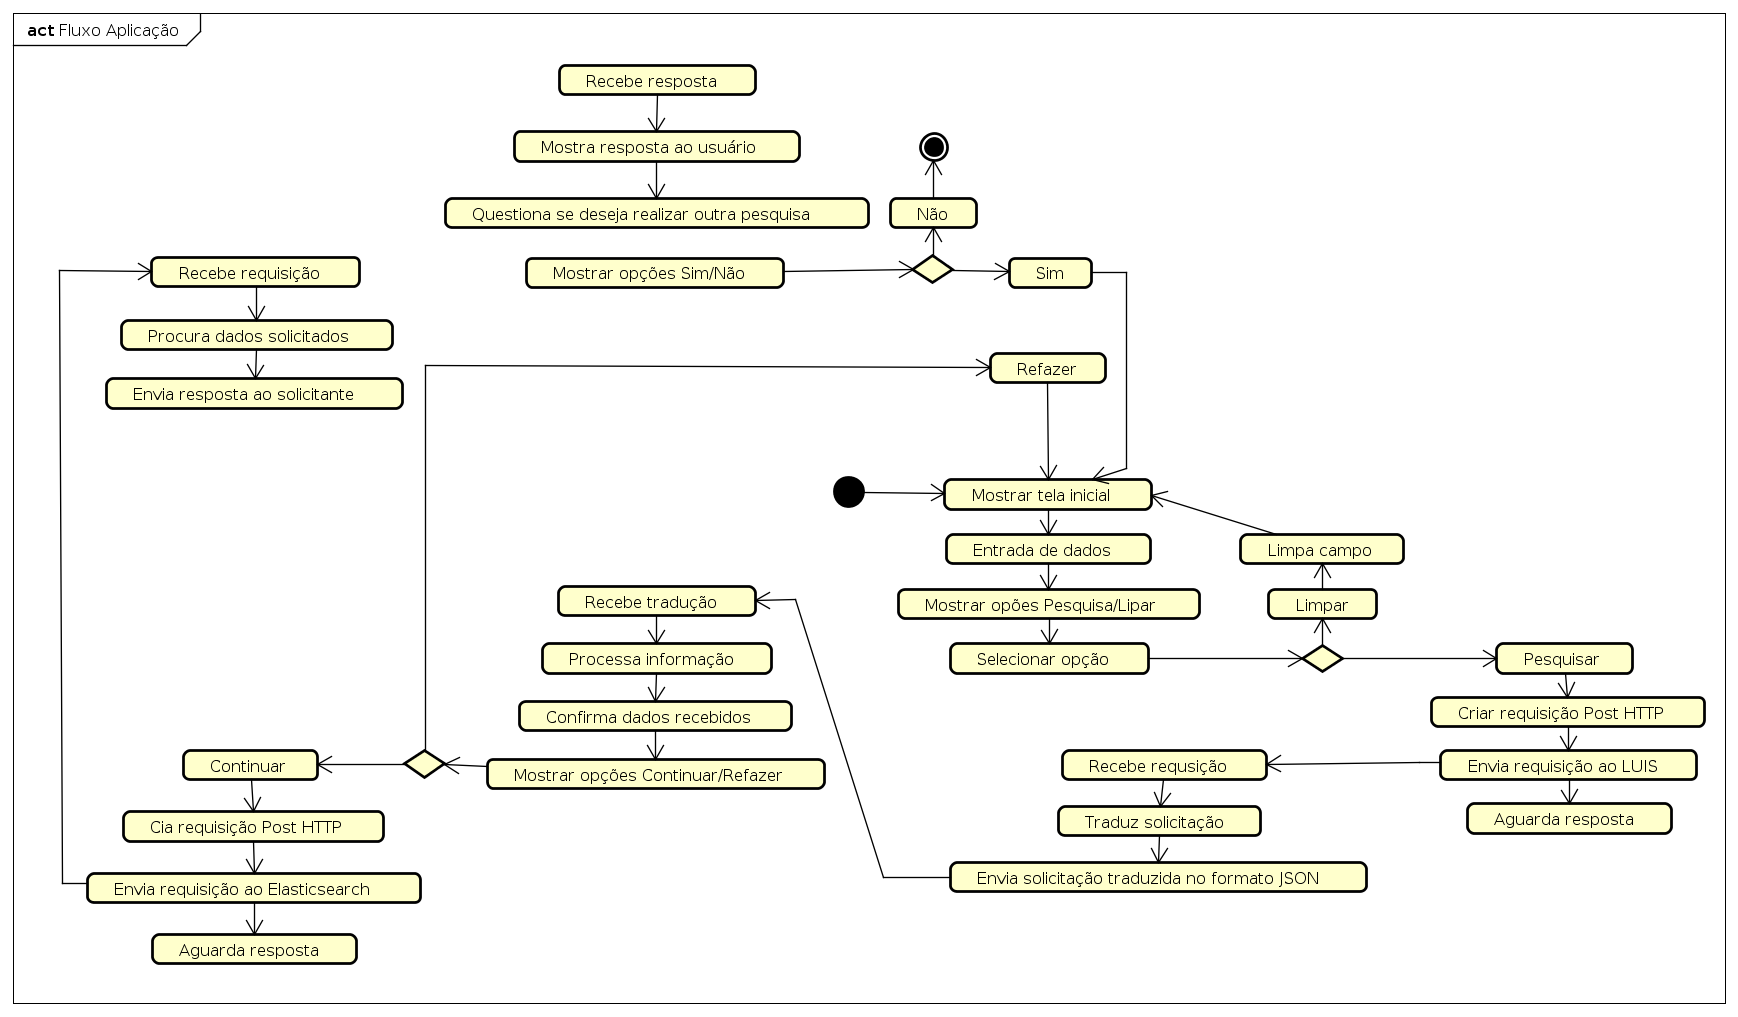
\includegraphics[angle=90, width=\textwidth, height=\textheight]{imagens/diagfluxo.eps}
        \end{center}
        \legend{Fonte: Autor}
\end{figure}
